
\label{ch:Implémentations aristiques}

\section{Introduction}

Cette section conclut un point de vue artistique sur les aspects abordés dans les chapitres précédents. À partir de la transformation de Fourier en vocodeur de phase et en passant au morphing par des interprétations artistiques des patchs techniques mis en œuvre. Pour finir, on va utiliser un sous-ensemble du code écrit pour composer une pièce démonstrative de l'univers sonore abordée par le vocodeur de phase.

L'objectif de ce chapitre est de soutenir l'idée que l'analyse spectrale et la re-synthèse spectrale, sont utiles aux scientifiques et aux artistes. Donc, par extension, le développement du processus informatique du signal musical peut l'être aussi. En effet, les détails techniques antérieurs sont utilisés à des fins artistiques et esthétiques. Les exemples suivants consistent en une expérimentation personnelle et une interprétation du matériel technique déjà présenté.

\section{Le vocodeur de phase - \textit{Une capacité sans fin}}

\subsection{Super Phase Vocoder}

Dans le but de combiner plusieurs techniques du vocodeur de phase, nous avons implémenté un \guillemotleft \textit{super} vocodeur de phase\guillemotright . Cet outil spectral comprend l'étirement temporel, le freeze temporel, le décalage de hauteur, le morphing et d'autres effets bénéficiant de la fonction élémentaire du vocodeur de phase.

Le graphe \ref{FirstMorphingTry} présente le patch de contrôle de tous les paramètres du vocodeur de phase. Cette version du vocodeur de phase contient tous les effets étudiés dans les sections précédentes. La différence entre le patch du vocodeur de phase de base pour le morphing est minime. Essentiellement c'est le même code avec quelques fonctionnalités supplémentaires. Il est naturel de rechercher une fonctionnalité plus large pour le même outil. En suivant cette raisonnement, nous avons implémenté tous les effets de base dans un seul patch. Les formules mathématiques correspondantes à ce partie sont omises car nous les avons déjà balayées auparavant. Les détails les plus cruciaux se trouvent dans la séquence de tous les effets visibles dans figure \ref{SuperPhaseVoc}.

Dans le patch principal, vous pouvez voir deux pianos virtuels de contrôle permettant de modifier la hauteur de chaque son séparément. Idéalement, ce système devrait être automatique. Il faut estimer la fréquence de chaque son et corriger à mi-chemin la hauteur du son pour qu'il en soit de même. Une correction de hauteur intervient avant tout effet de morphing et n'affecte donc pas le résultat. Dans le patch principal, nous pouvons également trouver des commandes permettant de manipuler le filtre de Gabor, en ajustant les composantes de bruit de la phase qui, dans ce patch, sont identiques pour les deux sons. On peut également trouver des facteurs d’interpolation de magnitude et de phase pour le morphing, ainsi que la factorisation de la courbe, comme indiqué dans la section précédente. La dernière modification présentée dans ce patch est l'effet de \textit{freeze} qui contient les valeurs spectrales d'une seule fenêtre. Pour cet effet, deux types de filtrage sont également ajoutés pour modifier le timbre des spectres gelés.


\begin{figure}
\centering
\begin{subfigure}{\textwidth}
  \centering
  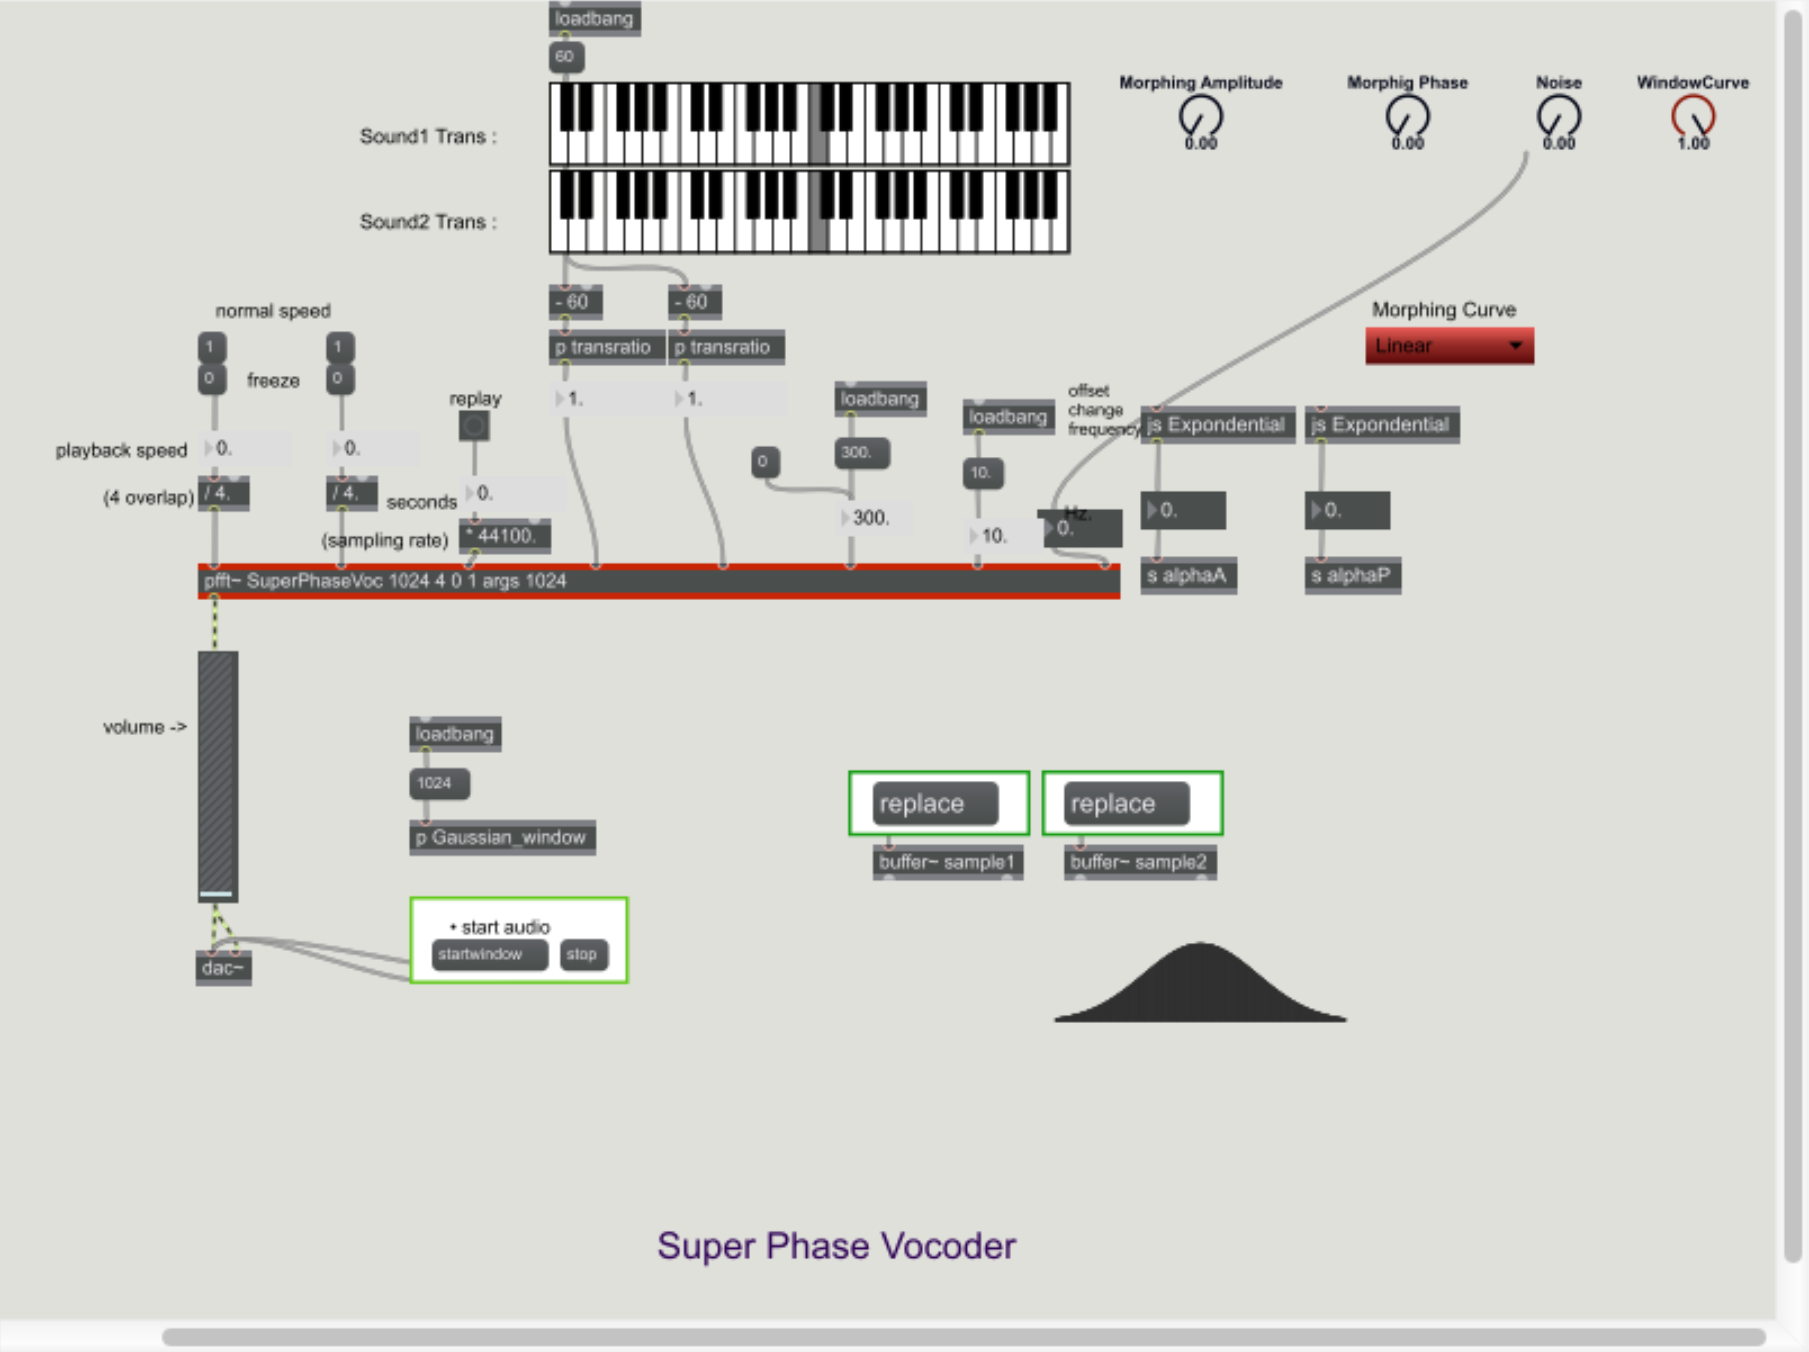
\includegraphics[width=.8\linewidth]{Graphs/FirstMorphingTry.png}
  \caption{Super Phase Vocoder I}
  \label{FirstMorphingTry}
\end{subfigure}

\begin{subfigure}{\textwidth}
  \centering
  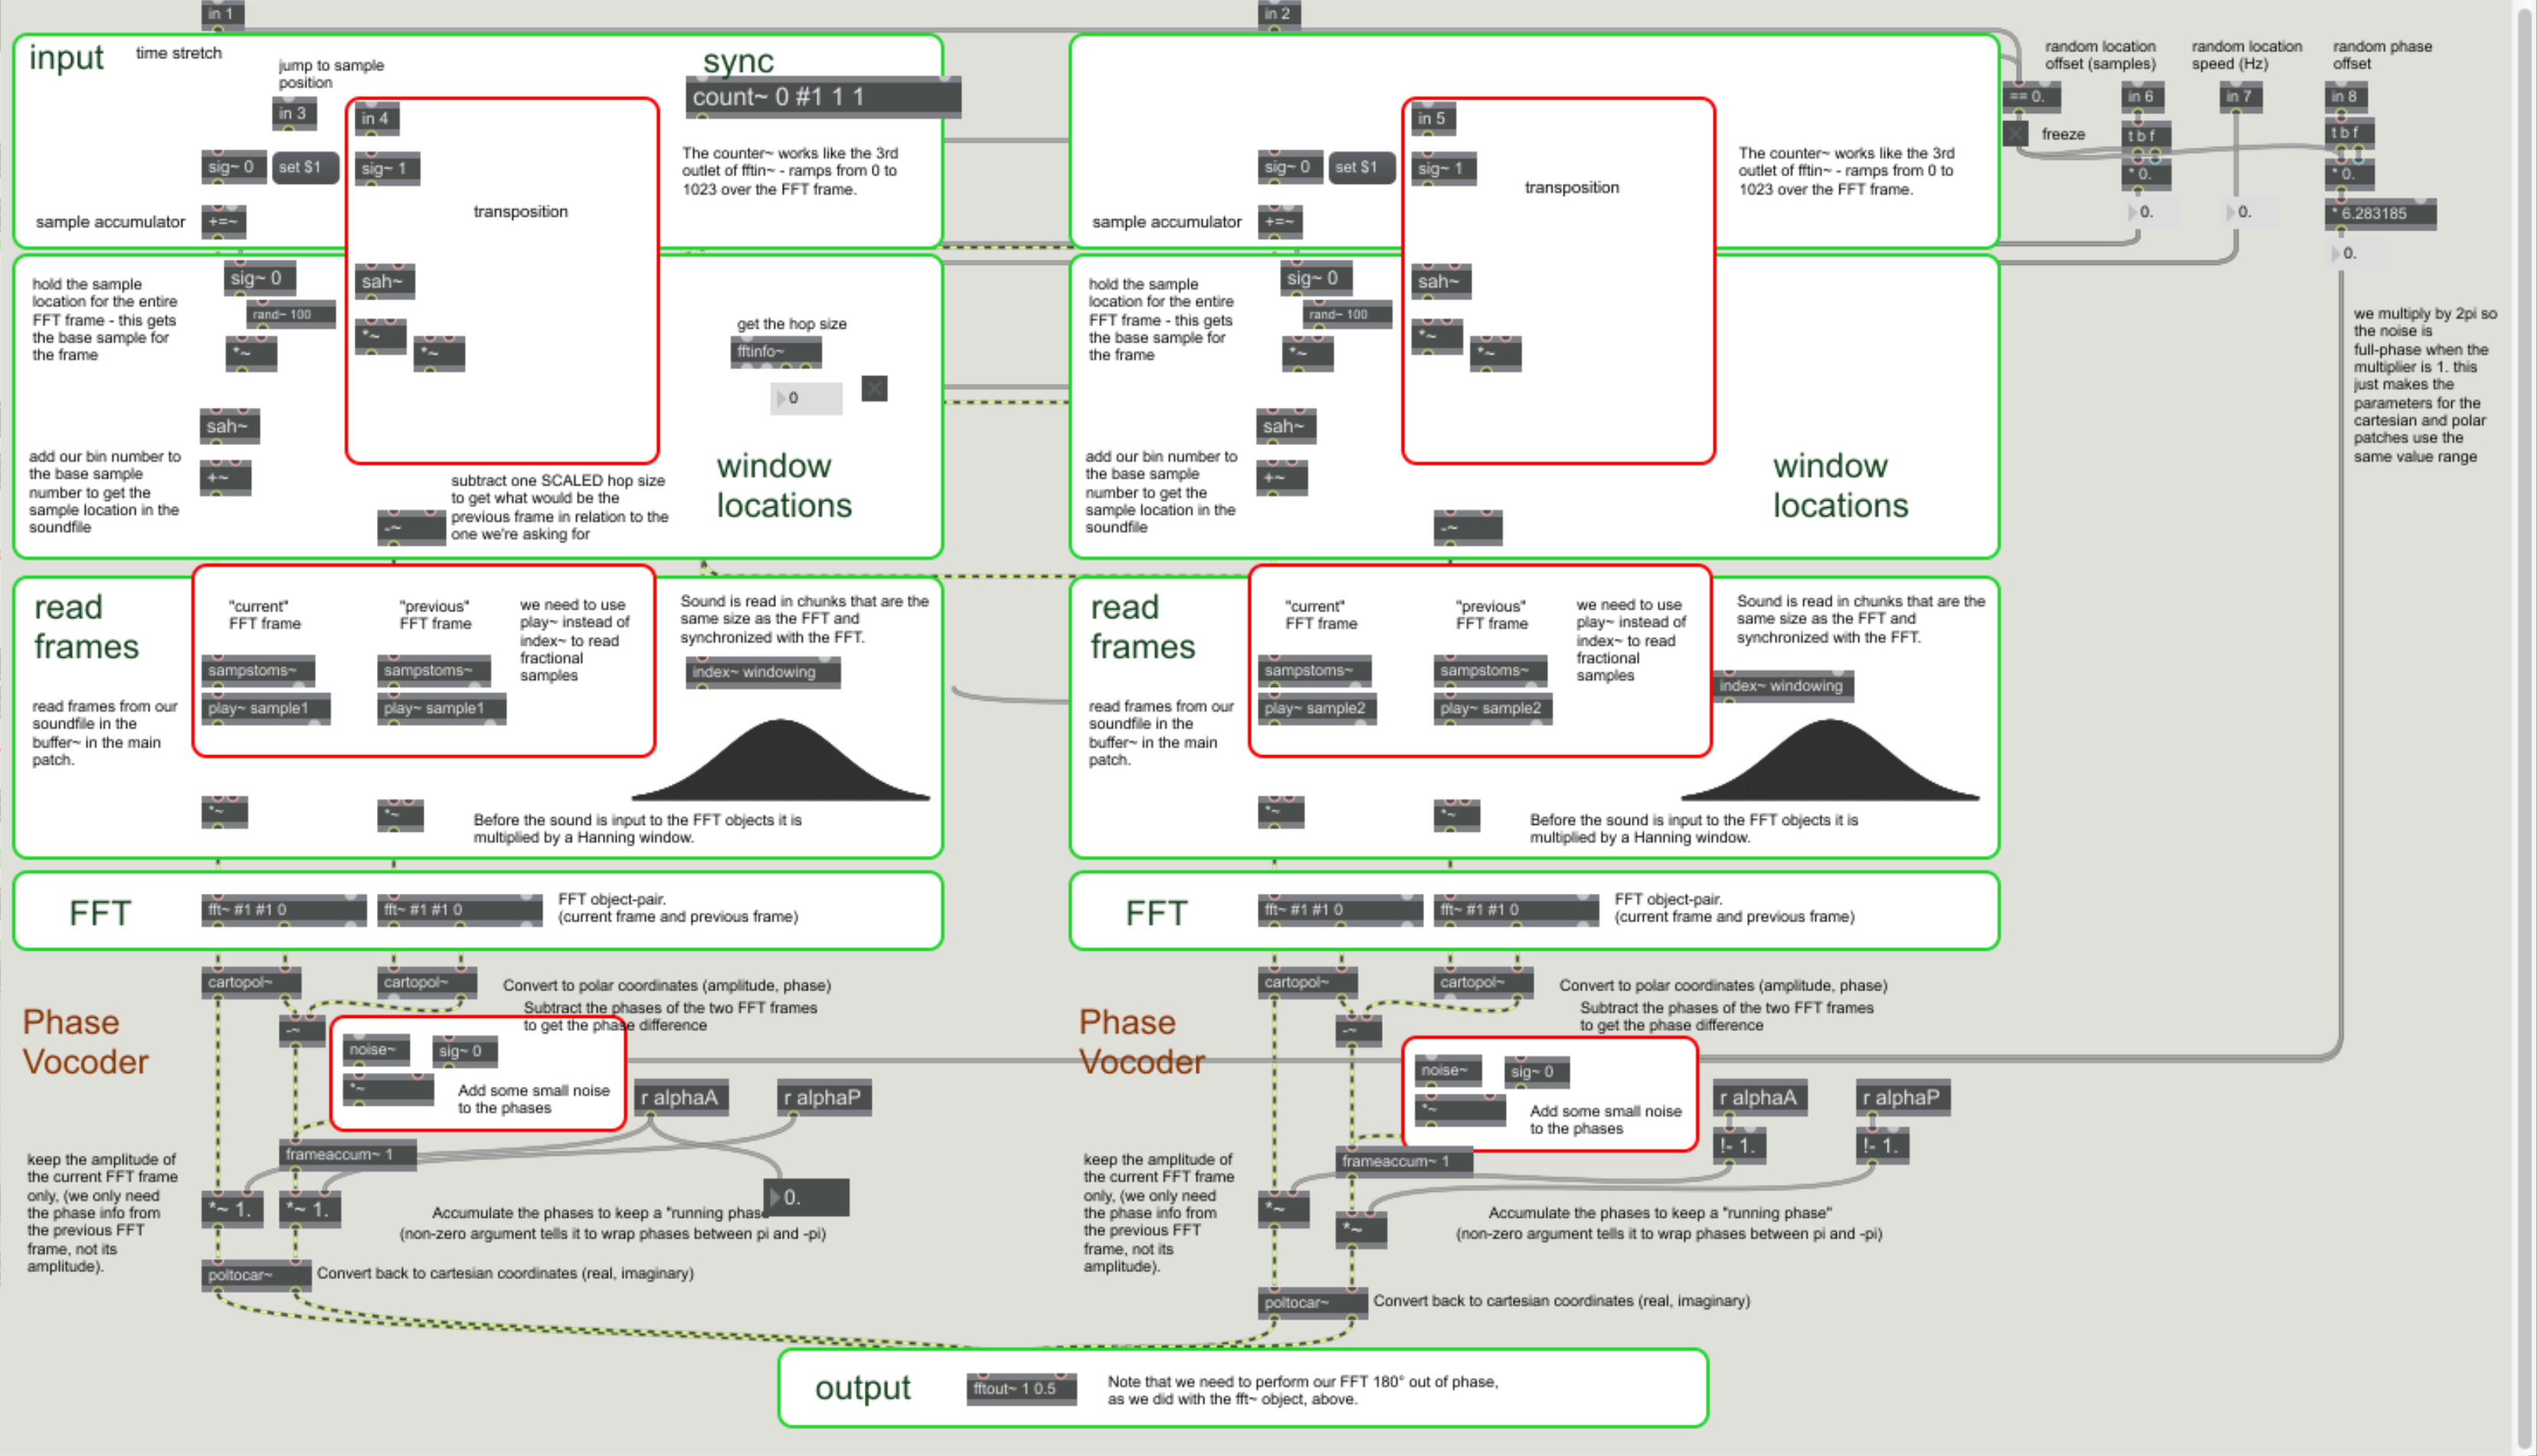
\includegraphics[width=.8\linewidth]{Graphs/SuperPhaseVoc.png}
  \caption{Super Phase Vocoder II}
  \label{SuperPhaseVoc}
\end{subfigure}
\caption{Super Phase Vocoder}
\label{PhaseVocoder}
\end{figure}

\subsection{l'interférence de phase}
    Dans ce patch Max, nous étudions une modification des coordonnées polaires après l’étape de l’analyse. Nous ajoutons simplement un oscillateur \textit{phaser}$\thicksim$ après la FFT et l’appliquons à chaque amplitude et phase corrigée de la fenêtre. De cette façon, l'identité du signal n'est pas modifiée, mais une fréquence oscillante interfère avec chaque index de la fenêtre FFT. La formule de cette modification est présentée ci-dessous par l'équation de synthèse.

\begin{figure}
  \centering
  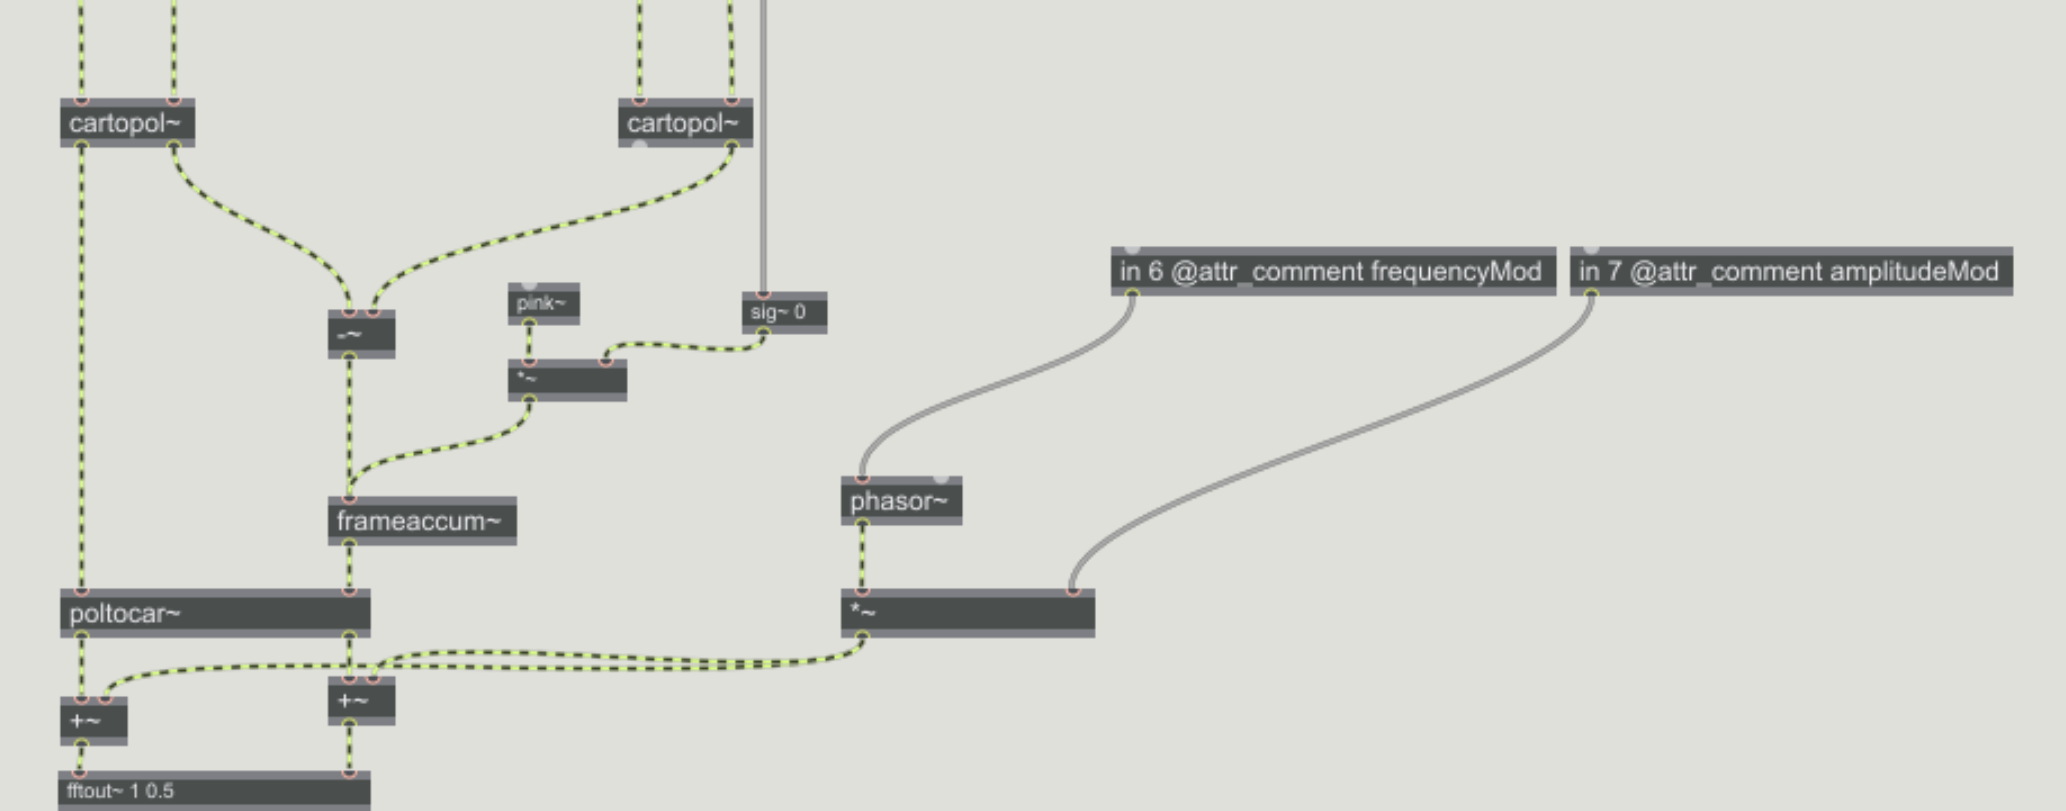
\includegraphics[width= 0.5 \textwidth]{Graphs/phasorInt.png}
  \caption{modulation \\ des coordonées polaires}
  \label{phasorInt}
\end{figure}

    \begin{equation}
      y(n, k) = \sum_{k=1}^K (A[n]+phi(n)) \; e^{j (\theta_k(n) +\phi(n)}
    \end{equation}
    
    Où $y (n, k)$ est le signal fenêtré après l'analyse. K est le nombre de sinusoïdes, $ A [n] $ est la magnitude instantanée, $ \theta $ est la phase instantanée et $ \phi (n) $ est le phaseur instantané donné par la formule:

    \begin{equation*}
        \phi(n) = n - floor(n)
    \end{equation*}

    Nous pouvons voir que le modèle sous-jacent de la FFT est utilisé pour représenter cette modification. D'autres modèles pourraient parfaitement décrire cet effet, mais dans cette version, il est plus direct. Dans la figure correspondante \ref{phasorInt}, nous pouvons voir le phaseur moduler la magnitude et la phase. La fréquence et l'amplitude du phaseur sont contrôlées dans le patch principal contenant l'objet \textit{pfft$\thicksim $}.

\subsection{Modulation au bruit}

    Dans ce vocodeur de phase, nous étudions une modulation de bruit sur la composante de fréquence. Nous avons ajouté la composante de bruit et essayé différents générateurs de bruit tels que \textit{rand$\thicksim $}, pink-noise, white-noise et au même moment nous avons contrôlé le facteur d'amplitude de cette composante. Le sous-patch pour la sélection du bruit est visible dans la figure \ref{Noise_Select}. Un objet \textit{umenu} fonctionne comme un stade de sélection pour l'utilisateur transmettant ses valeurs au sous-patch pfft.

    La phase corrigée, par la fenêtre FFT de chevauchement, est multipliée par le facteur du bruit. Dans les dossiers sonores de cette thèse, on entend les différentes modulations de bruit, mais le résultat sonore n’est pas évident. Le facteur de bruit est utilisé pour la naturalisation du son car les fréquences continues pures ne sont pas produites dans les sons réels. Par conséquent, une petite correction de l'oscillateur de bruit ne donne pas un résultat strictement différent.

\begin{wrapfigure}{r}{0.4\textwidth}
  \vspace{-20pt}
  \begin{center}
    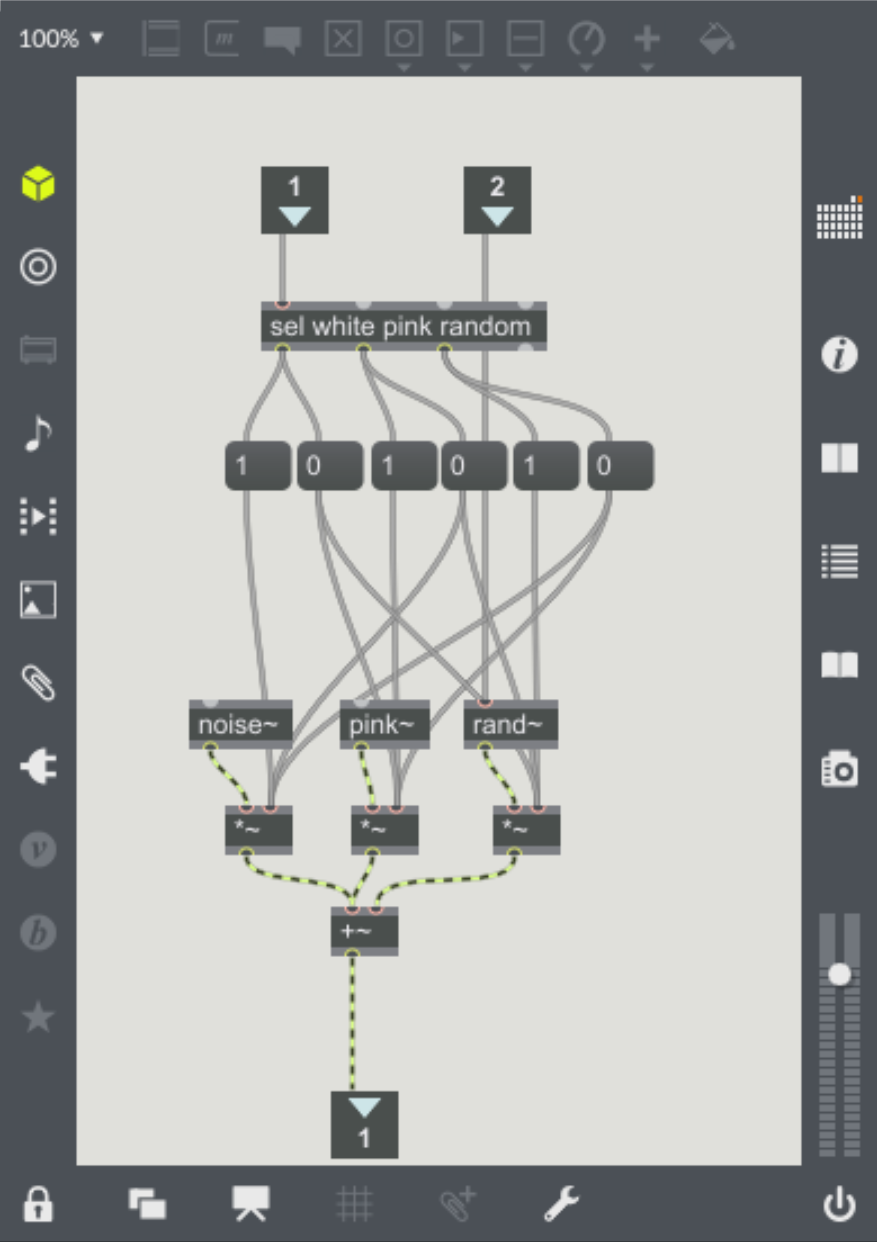
\includegraphics[width=0.48\textwidth]{Graphs/Noise_Select.png}
  \end{center}
  \vspace{-20pt}
  \caption{Selection du bruit}
  \vspace{-10pt}
\end{wrapfigure}

\subsection{Filtre aléatoire sur la position du buffer$\thicksim$}

    Dans ce patch, nous modulons la position du tampon via un générateur de signaux aléatoires qui transmet ses valeurs au lecteur de la position du fichier. Pour être plus précis, nous filtrons les harmoniques de la FFT en produisant des nombres aléatoires pour chaque harmonique et en ne calculant l'harmonique $ k-$\ième que si le nombre aléatoire correspondant est inférieur à sa valeur d'index.
    
    \begin{figure}
        \centering
        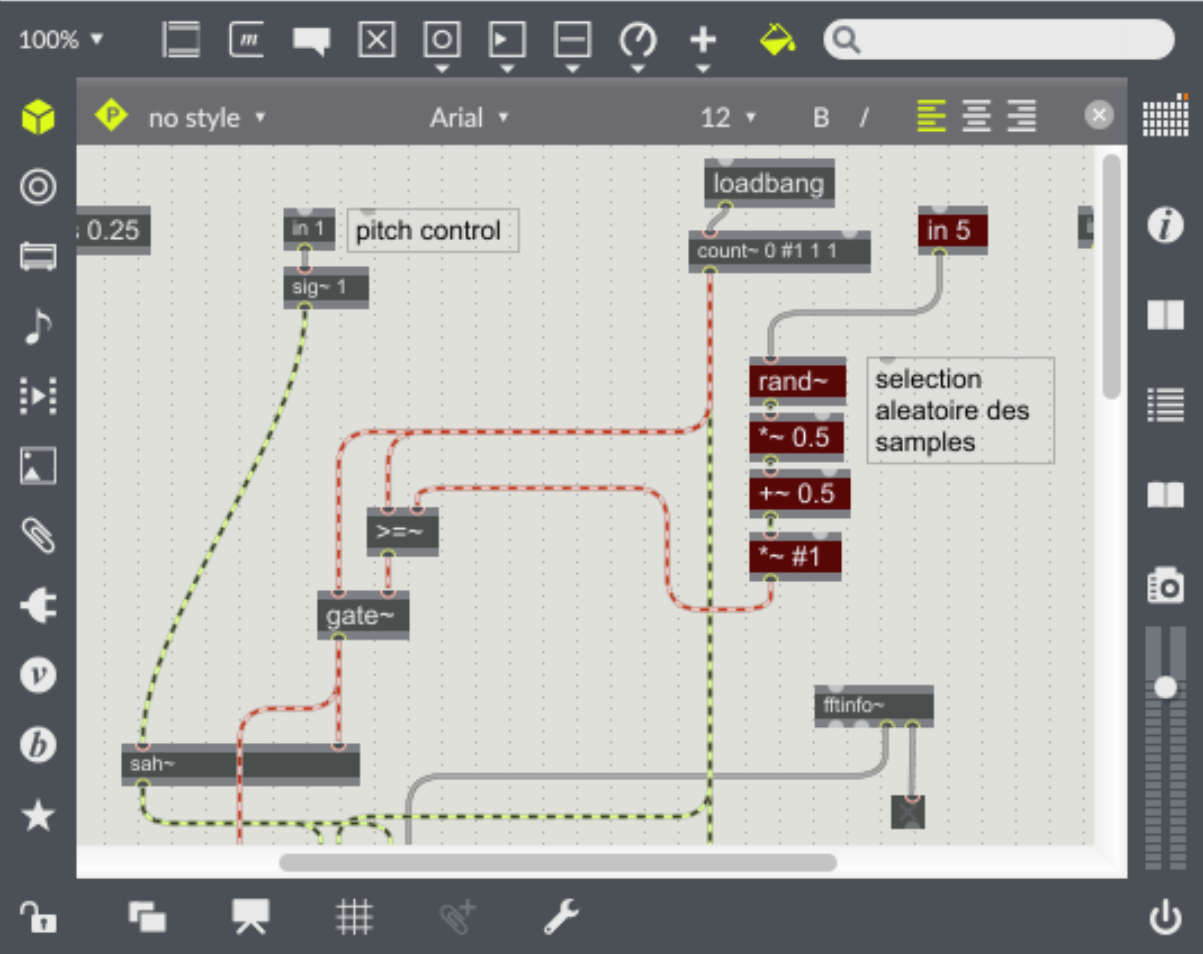
\includegraphics[width = 0.4 \textwidth ]{Graphs/random_sampling.png}
        \caption{Filtre aléatoire}
        \label{FiltreAleatoire}
    \end{figure}

% \begin{wrapfigure}{r}{0.5\textwidth}
%   \vspace{-20pt}
%   \begin{center}
%     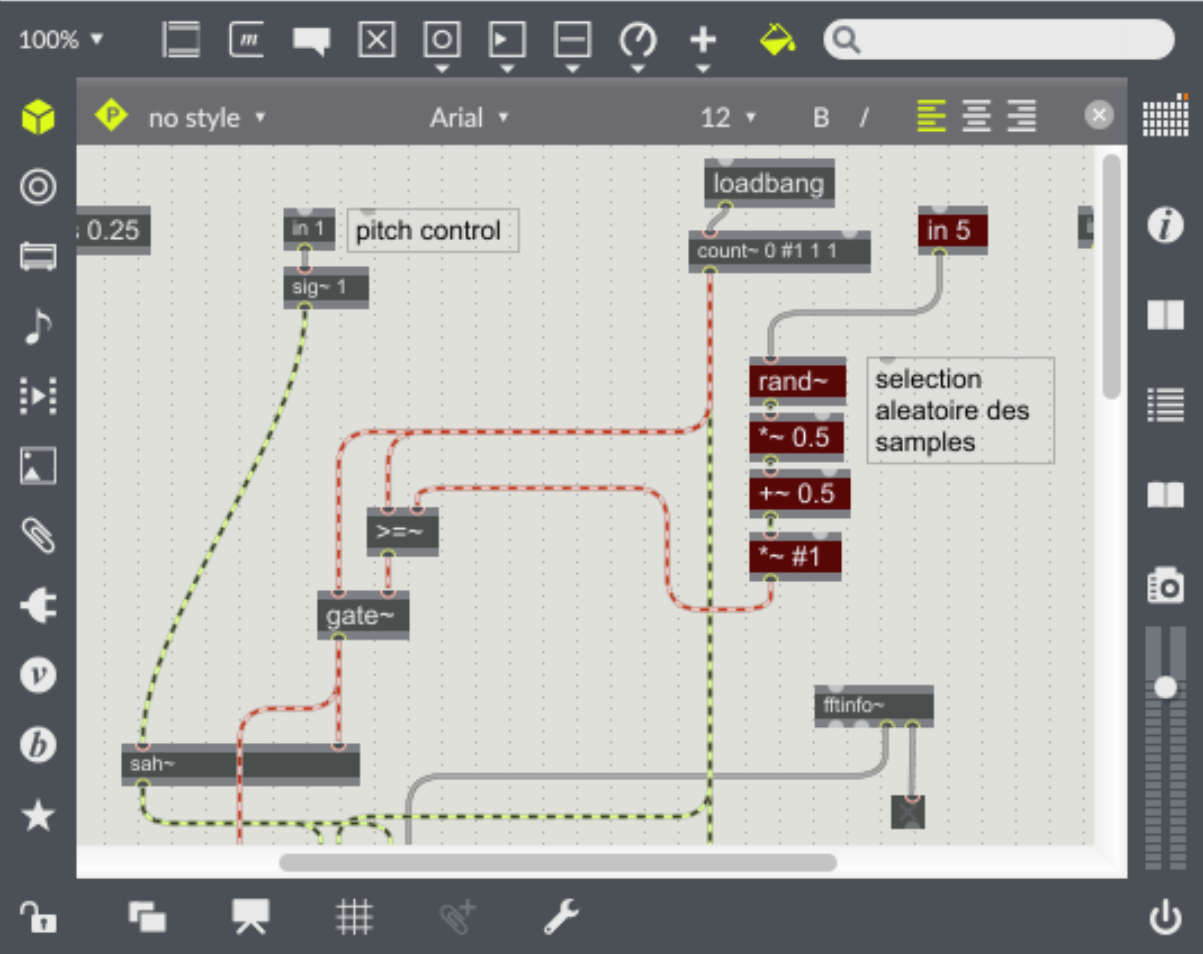
\includegraphics[width=0.48\textwidth]{Graphs/random_sampling.png}
%   \end{center}
%   \vspace{-20pt}
%   \caption{Filtre aletoire}
%   \vspace{-10pt}
% \end{wrapfigure}

    Le générateur aléatoire est créé par l'objet \textit{random$\thicksim $} avec un filtre modulant la fréquence de la génération de valeur aléatoire. La valeur transmise au lecteur de l'objet \textit{play$\thicksim $} est modulée par un détenteur d'échantillon qui prend en entrée la sortie d'un compteur et la valeur générée de manière aléatoire. Le porte-échantillon est créé manuellement par un objet supérieur à un objet et une porte. De cette manière, nous conservons et publions de manière abstraite des valeurs dans la fenêtre FFT, créant ainsi un système hybride de modulation de la hauteur et de la lecture. La modulation peut être trouvée dans la figure \ref{FiltreAleatoire}.

\subsection{Robotisation}
    
\begin{wrapfigure}{r}{0.5\textwidth}
  \vspace{-20pt}
  \begin{center}
    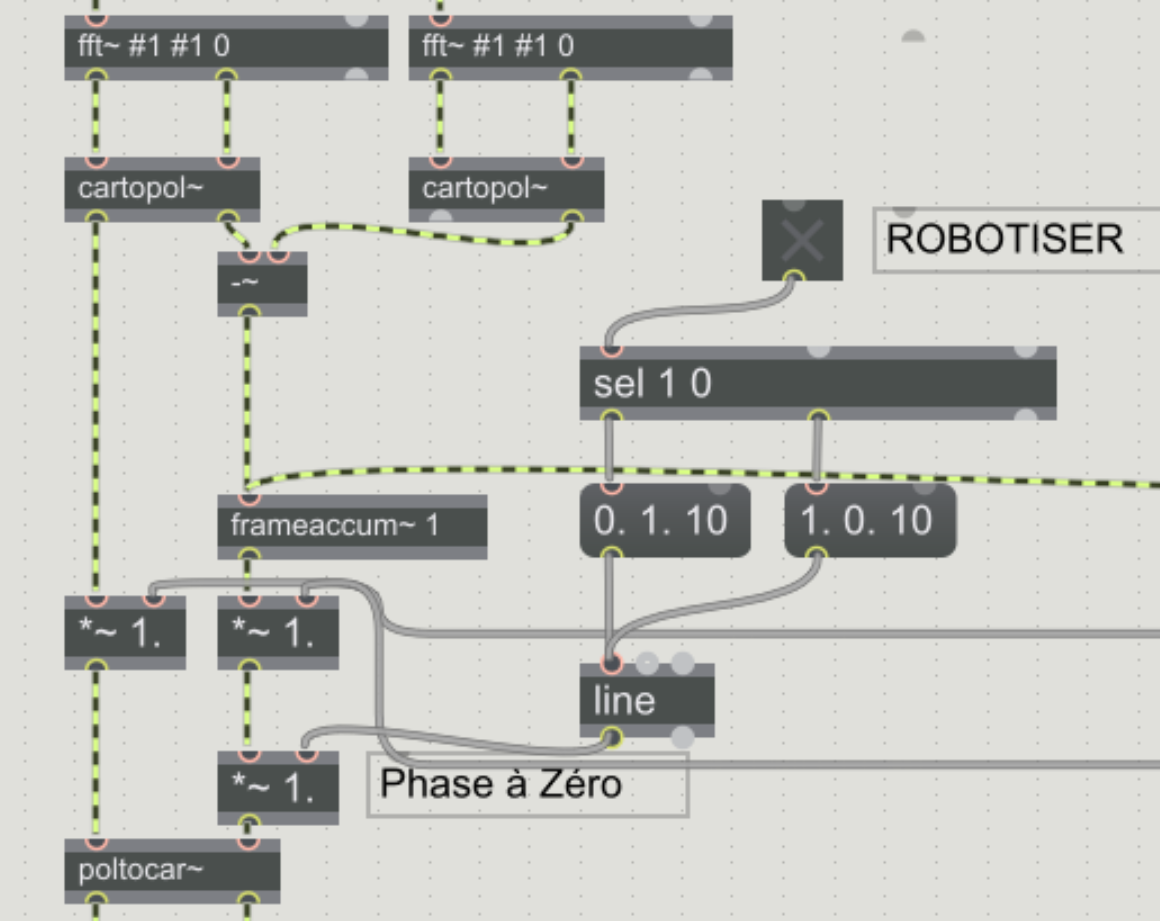
\includegraphics[width=0.48\textwidth]{Graphs/Robotisation.png}
  \end{center}
  \vspace{-20pt}
  \caption{Robotisation}
  \vspace{-10pt}
\end{wrapfigure}

    La robotisation est achevée par une modification sur la phase de chaque harmonique du vocodeur de phase pendant l'analyse. En effet, en mettant la phase de tout harmonique à zéro on garde que la magnitude. Cette technique permet d'avoir une phase incorrecte constante pour les partiels du son d'entré mais avec une amplitude correspondante variée.
    L'implementation est montré dans la figure.
  

\section{Morphing visuel}

En avançant sur le morphing visuel, nous avons implémenté le patch suivant avec l’aide du Jitter, pour une interpolation linéaire entre deux dessins.

    \begin{figure}
        \centering
        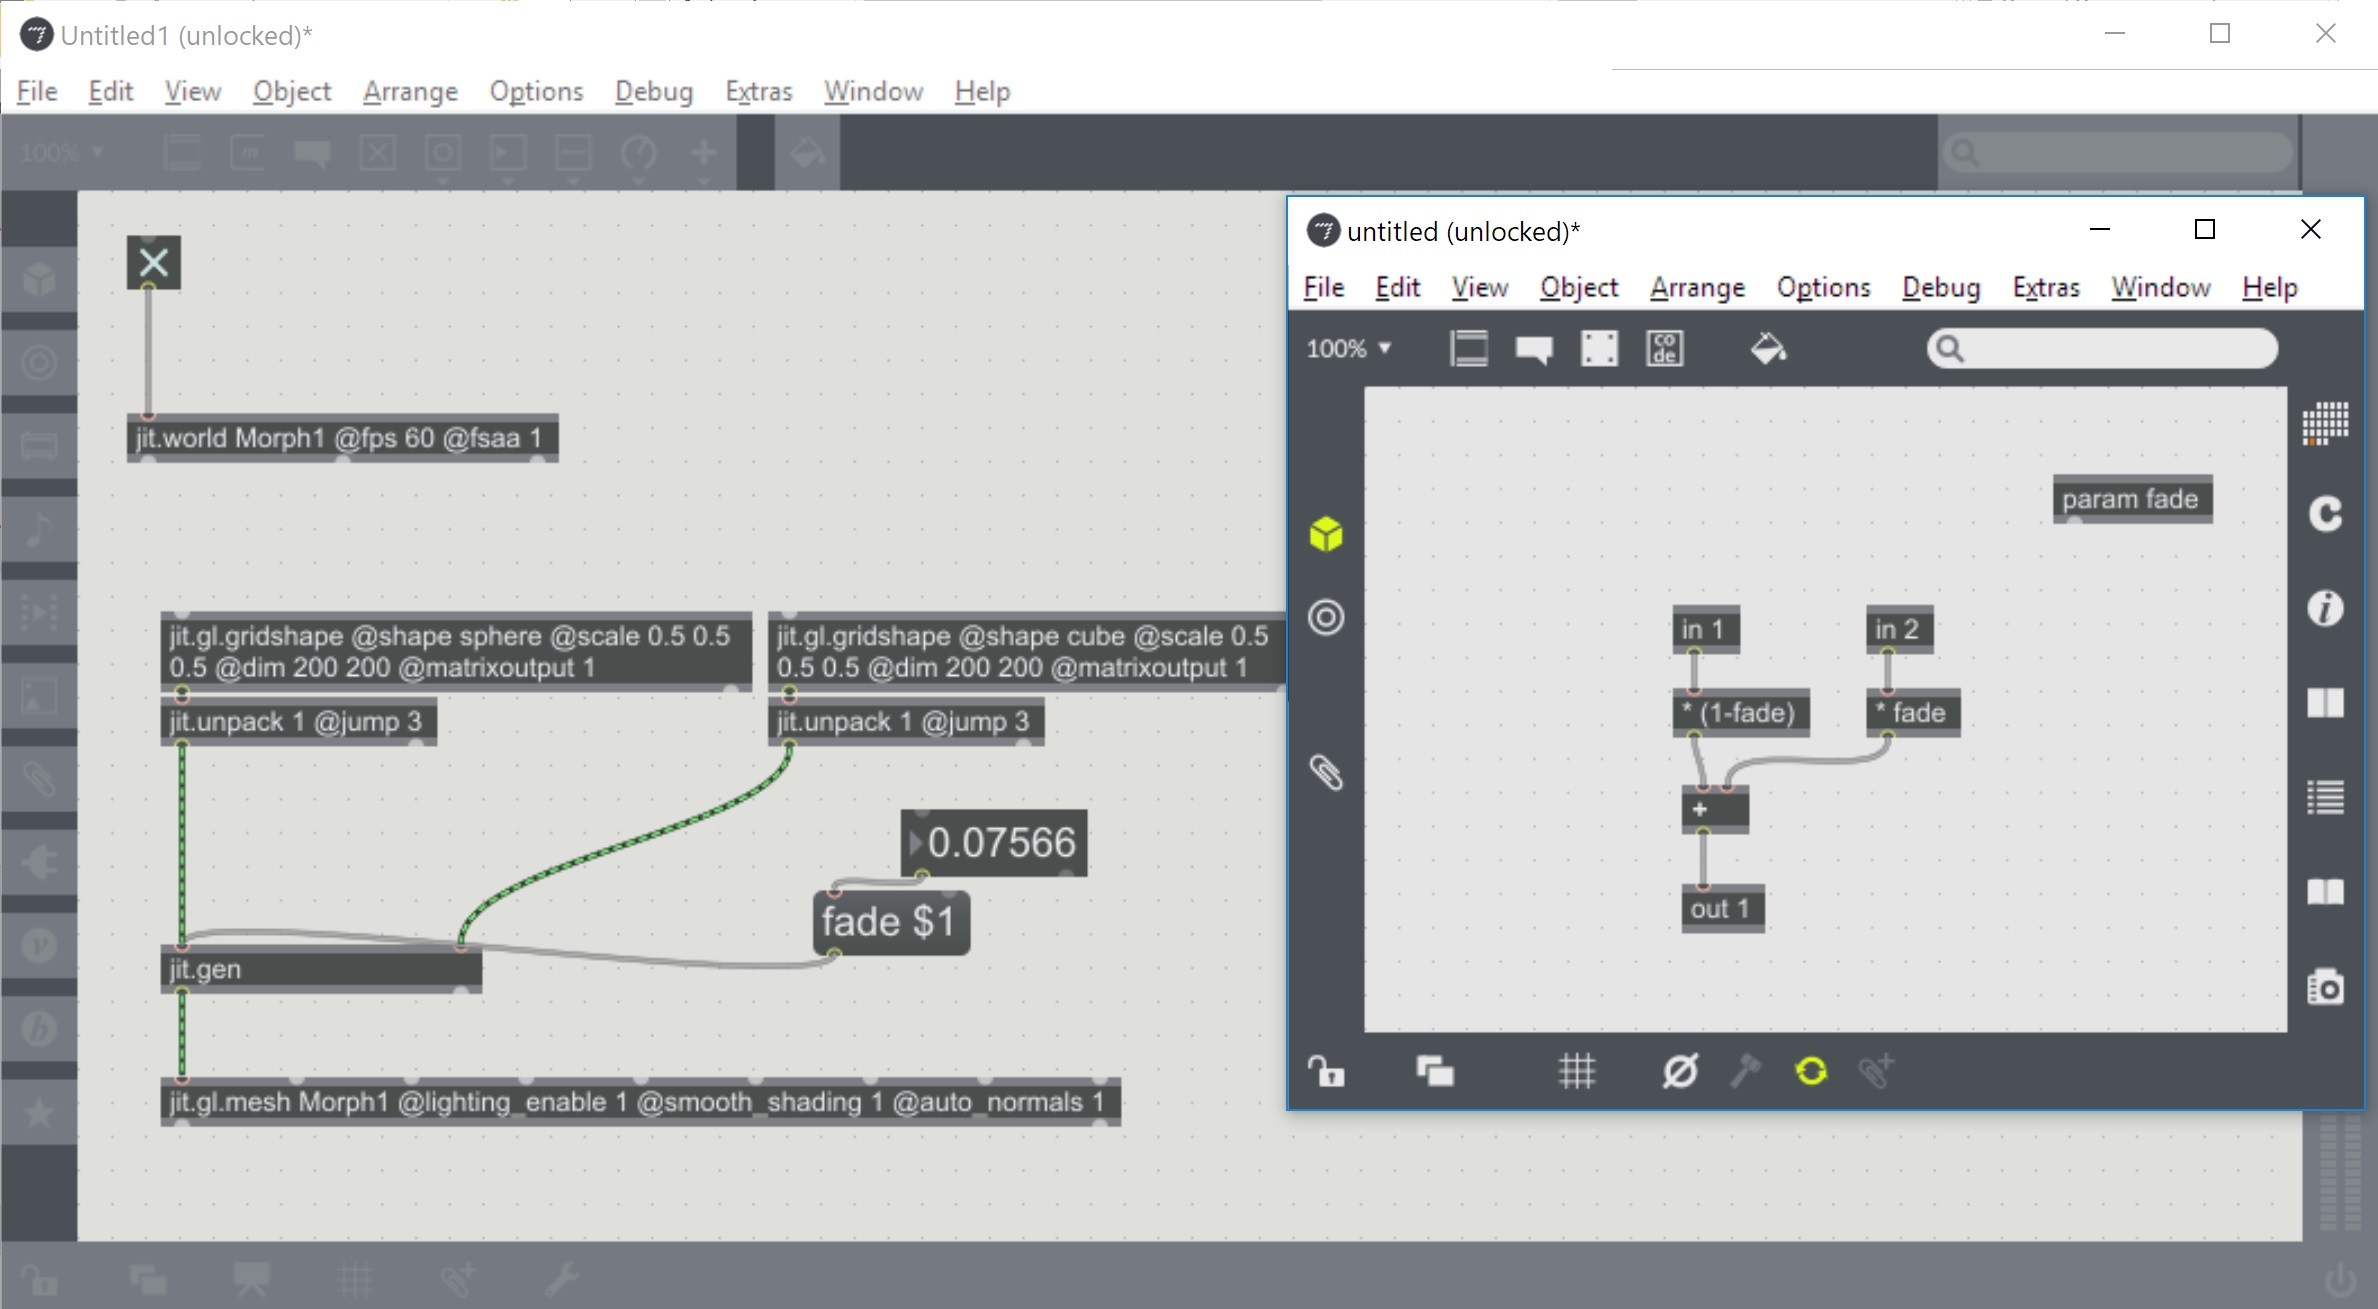
\includegraphics[width = \textwidth ]{Graphs/Morphing_patch.jpg}
        \caption{Visual Morphing}
        \label{VisualMorph}
    \end{figure}


En répétant la formule de base de morphing $M(\alpha) = \alpha\widehat {S_1} + [1 -\alpha]\widehat {S_2} $ une patch sur le morphing en 3D était implémenté avec l'aide de l'objet jit.gen (figure \ref{VisualMorph}).

Fondamentalement, le morphing visuel est relativement facile à réaliser avec les fonctions 3D primordiaux de Jitter telles que jit.gl.gridshape et jit.gen pour une personnalisation de la procédure de morphing. L'objet jit.gl.mesh est utilisé pour combiner le résultat du morphing alors que l'objet gen est contrôlé par un facteur de fondu.

À l'intérieur de gen, une procédure assez simple se produit. Les données multidimensionnelles provenant des matrices de localisation sont utilisées séparément pour chaque forme et leur amplitude est multipliée par le facteur $\alpha$ comme dans le morphing audio.

Bien entendu, nous pourrions également implémenter le script expondential.js pour une courbe de morphing différente sur le visuel.

Dans le patch suivant, nous avons voulu aller plus loin, en séparant tout composant d'un modèle tri-dimensionnel dans jitter. Nous distinguons les valeurs des matrices, des normals et de la texture. Nous avons ajoutés également une interpolation du couleur. Le patch est en disposition en figure \ref{VisualMorph2}.

    \begin{figure}
        \centering
        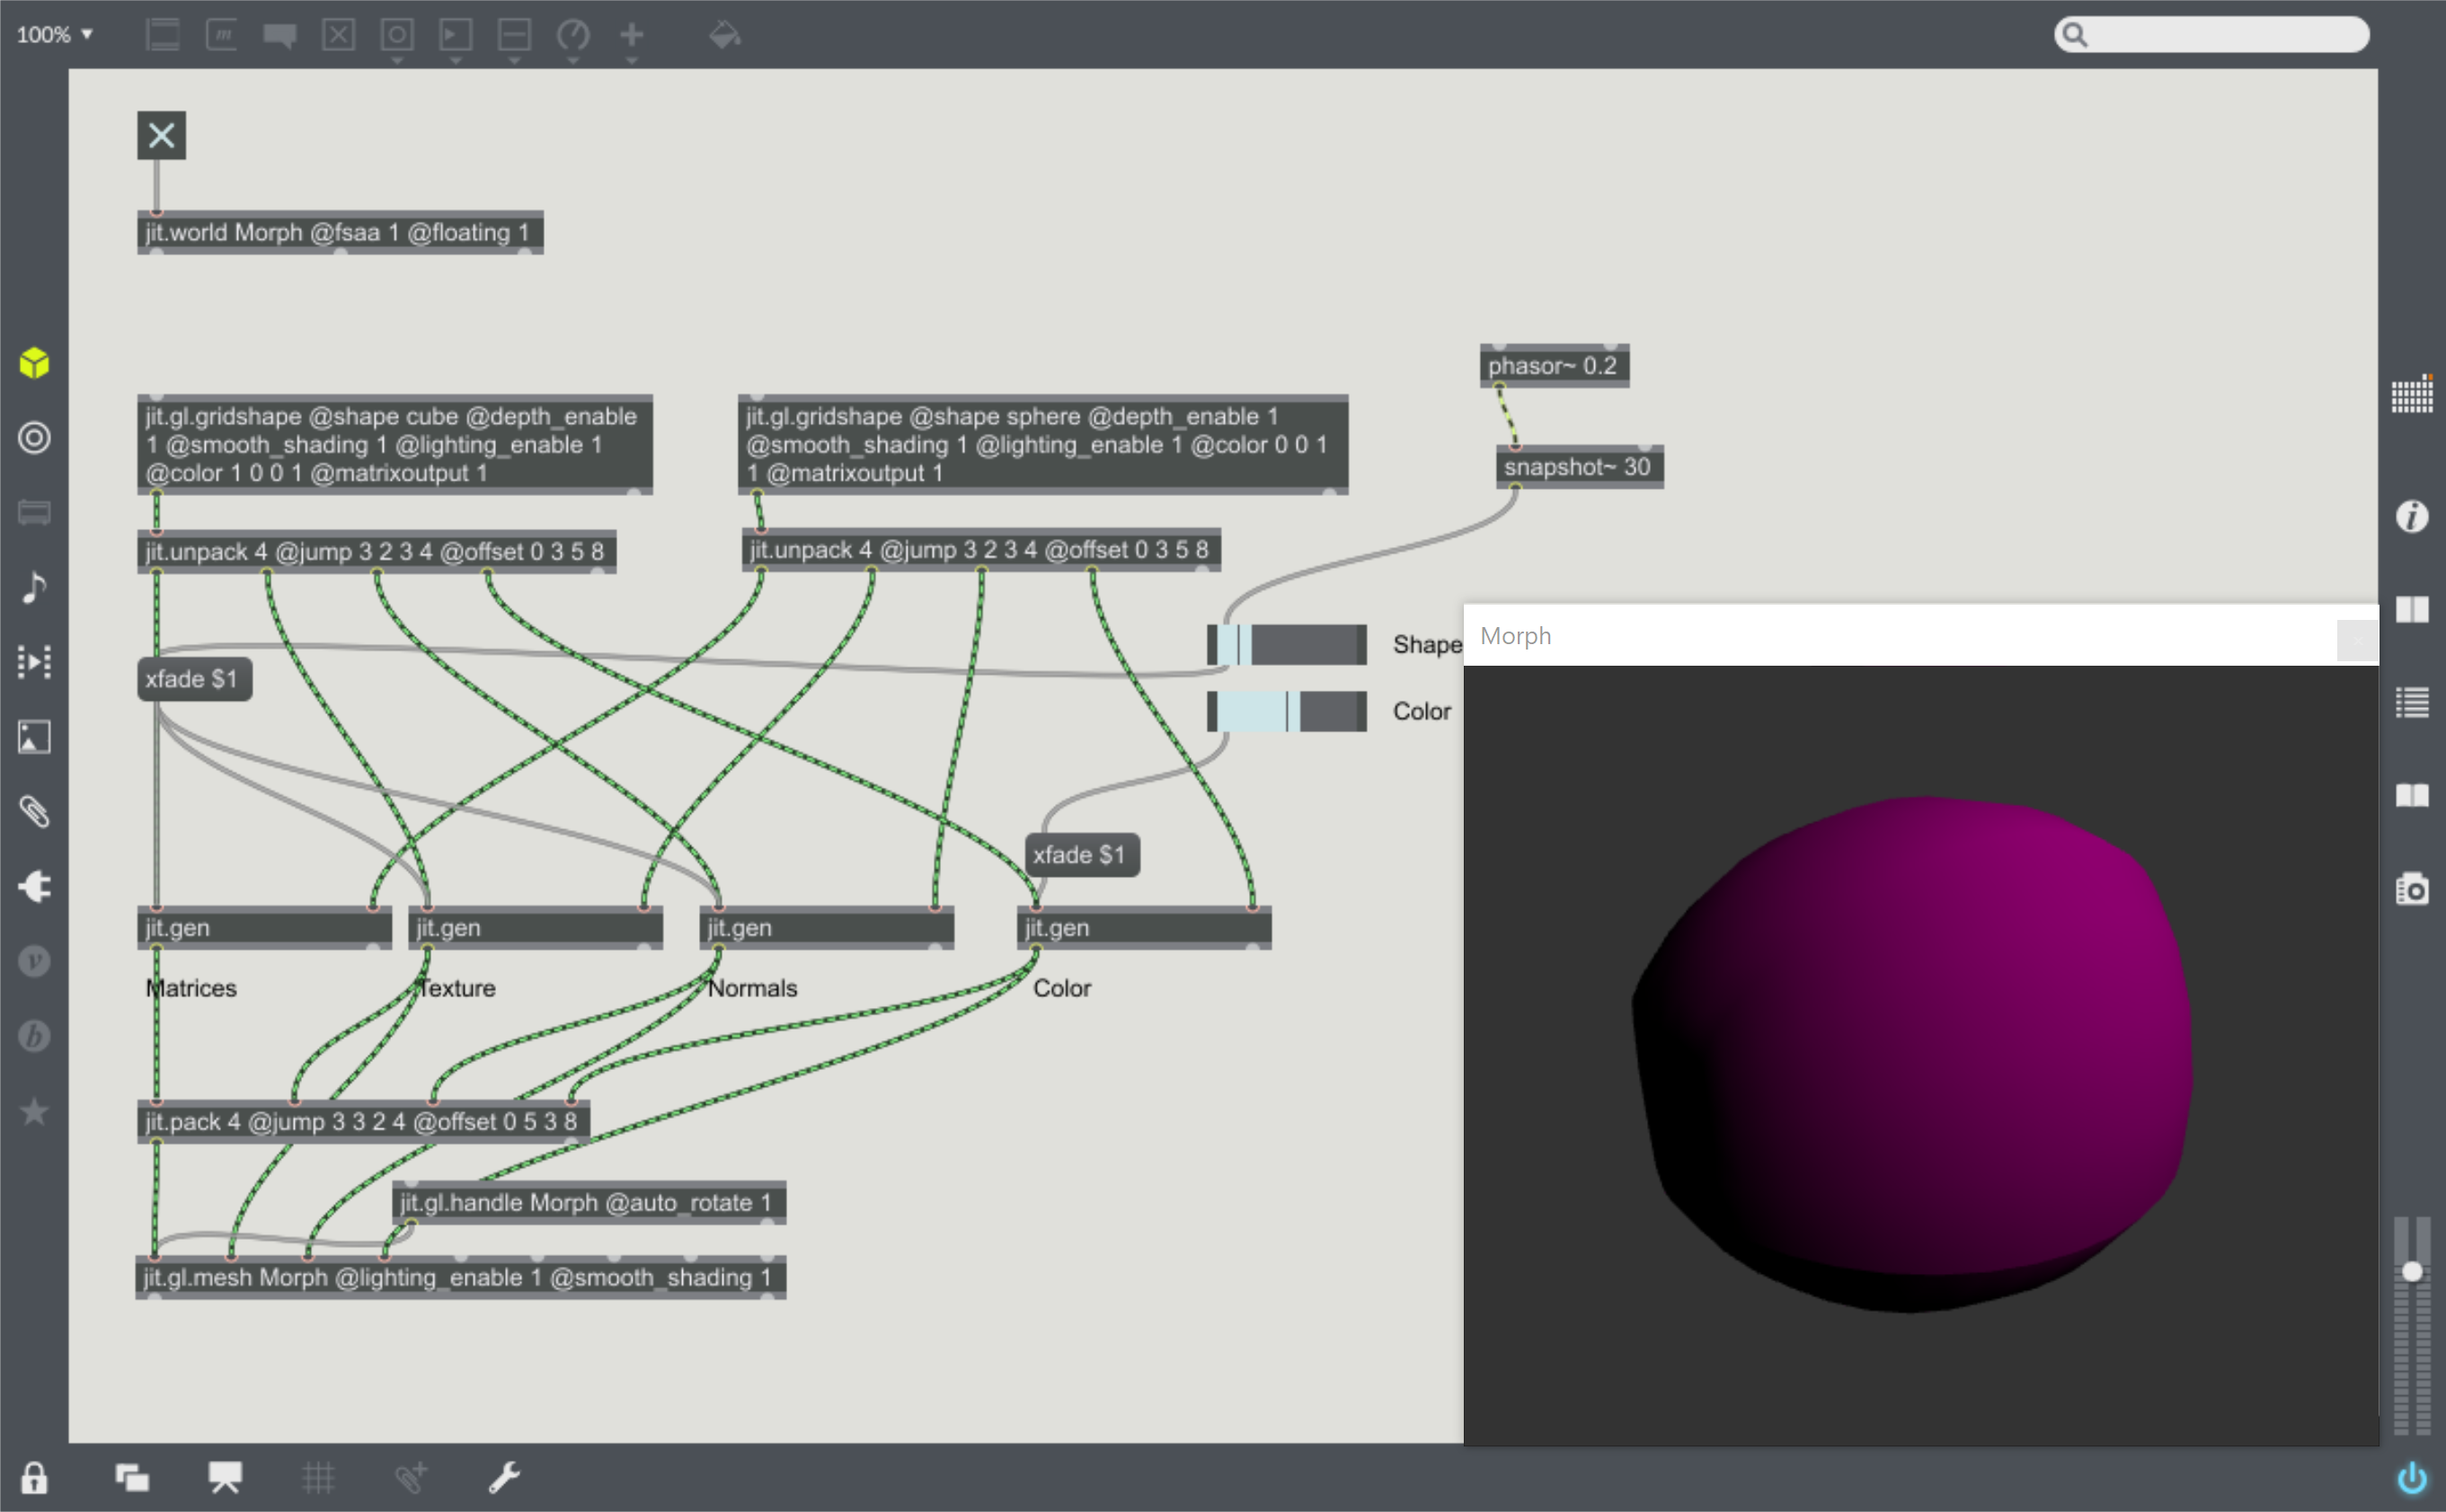
\includegraphics[width = \textwidth ]{Graphs/ShapeMorphing1.png}
        \caption{Visual Morphing $2^{ème}$ version}
        \label{VisualMorph2}
    \end{figure} 

\begin{figure}
\begin{subfigure}{.5\textwidth}
  \centering
  \caption{Interpolation de la forme : $0.0$ \\ Interpolation couleur : $0.0$}
  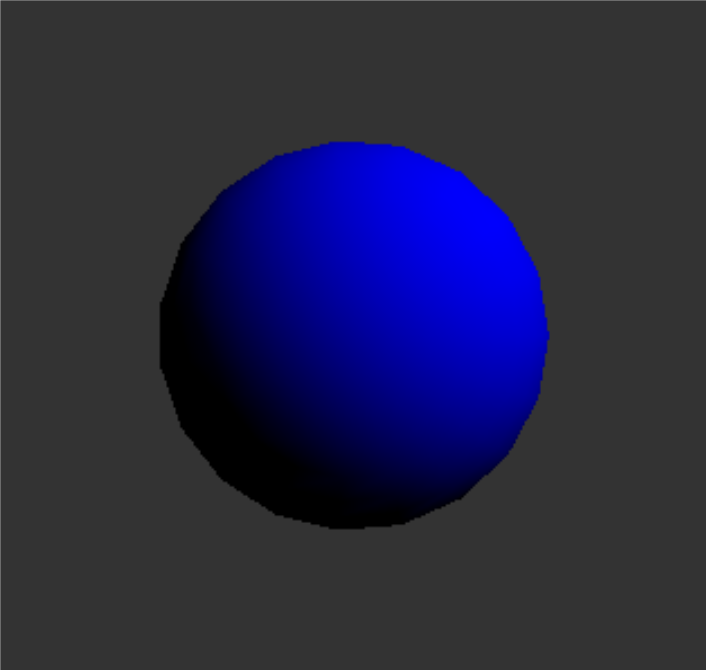
\includegraphics[width=1\linewidth]{Graphs/morph1.png}  
  \label{fig:sub-first}
\end{subfigure}
\begin{subfigure}{.5\textwidth}
  \centering
  \caption{Interpolation de la forme : $0.4$ \\ Interpolation couleur : $0.8$}
  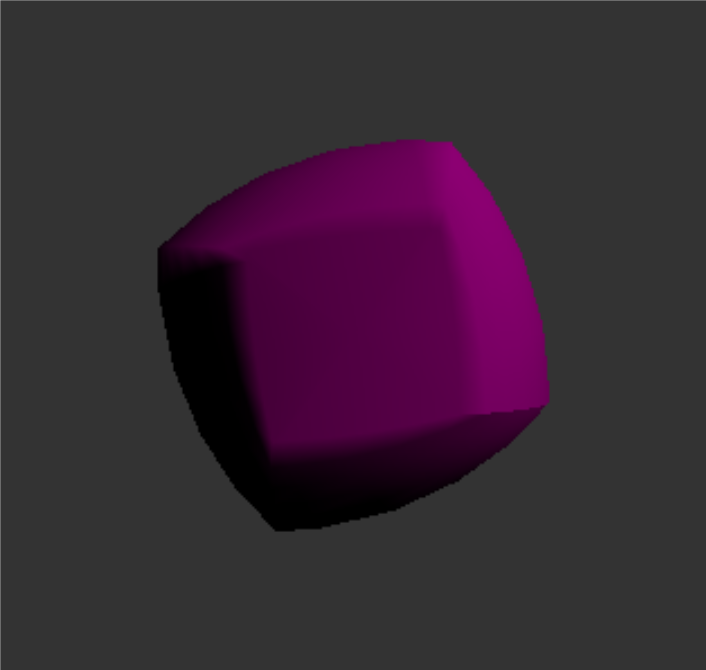
\includegraphics[width=1\linewidth]{Graphs/morph2.png}  
  \label{fig:sub-second}
\end{subfigure}

\begin{subfigure}{.5\textwidth}
  \centering
  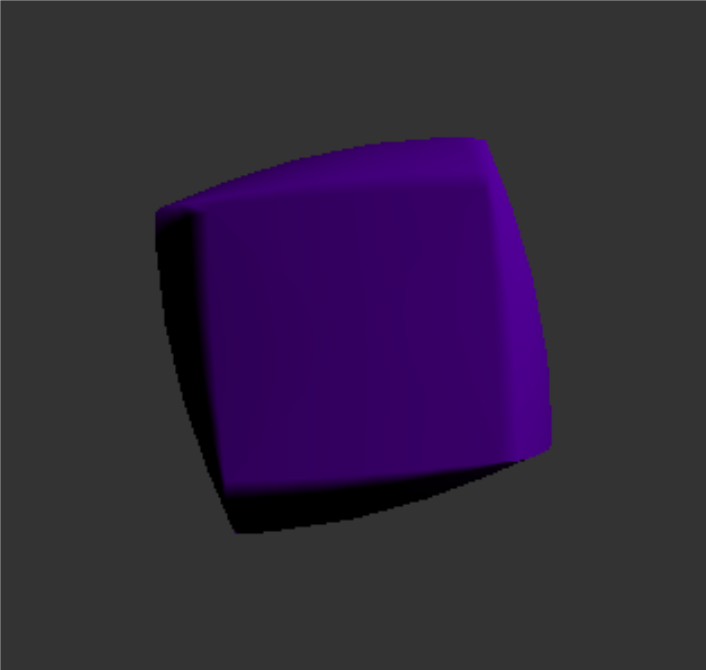
\includegraphics[width=1\linewidth]{Graphs/morph3.png}  
  \caption{Interpolation de la forme : $0.8$ \\ Interpolation couleur : $0.4$}
  \label{fig:sub-third}
\end{subfigure}
\begin{subfigure}{.5\textwidth}
  \centering
  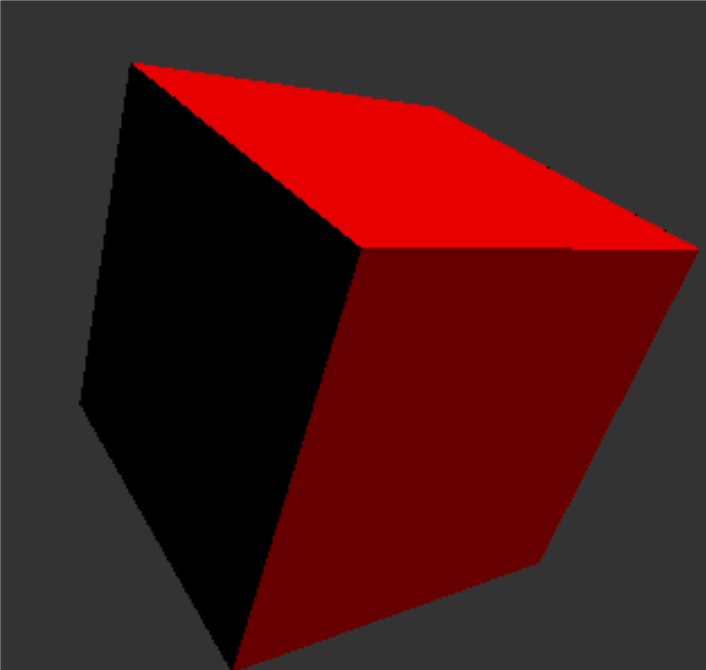
\includegraphics[width=1\linewidth]{Graphs/morph4.png}  
  \caption{Interpolation de la forme : $1.0$ \\ Interpolation couleur : $1.0$}
  \label{fig:sub-fourth}
\end{subfigure}
\caption{Stades du morphing visuel}
\label{fig:fig}
\end{figure}

\subsection{Visualisation du spectre}
    
    Dans ce patch, beaucoup de travail de Jitter a été implémenté à l'unisson d'un vocodeur de phase. Ce code permet de visualiser les informations spectrales d’un son sous la forme d’un paquet de lignes bidimensionnelles imitant les harmoniques trouvées lors d’une analyse de Fourier.

    Ce patch est utilisé en parallèle d'un vocodeur de phase pour le morphing ou même le simple décalage de pitch permet de visualiser l'évolution du spectre dans un environnement de rendu en temps réel. Dans ce code, nous utilisons une bibliothèque de jitter supplémentaire pour produire plusieurs objets jitter rendus dans un espace tridimensionnel virtuel. L'objectif de ce mémoire n'étant pas orienté sur l'image, nous ne dévoilerons, donc, que très peu d'informations sur le traitement présenté.

    Nous allons attribuer ici brièvement les objets les plus emblématiques du Jitter utilisés dans ce patch. L'objet \textit{jit.world} crée une nouvelle fenêtre et un espace de rendu virtuel tridimensionnel pouvant également contenir de la physique, des plans, des objets tridimensionnels, contrôler la position de la caméra, la couleur d'arrière-plan, etc. Le \textit{jit.gridshape} rend un objet tridimensionnel dans une fenêtre. La bibliothèque \textit{jit.mo} réplique de manière fluide les copies d’objets jitter. Et le \textit{jit.catch} prend un signal et le traduit en matrice jitter pour la visualisation potentielle.

    Pour transformer les informations spectrales en données tridimensionnelles, nous utilisons bien sûr une transformation FFT et un tampon qui lit les composantes polaires de la FFT (magnitude et phase) avec un objet \textit{peek$ \thicksim $} les envoie dans un tampon. Un objet \textit{lookup$ \thicksim $} récupère le contenu du tampon et les entre dans l'objet \textit{jit.catch}.

    Nous pouvons régler la dimension de \textit{jit.mo} pour générer plus d'harmoniques. Le son de sortie du vocodeur est envoyé à ce patch de visualisation harmonique pour saisir le résultat dans un espace 3D.


    \begin{figure}
        \centering
        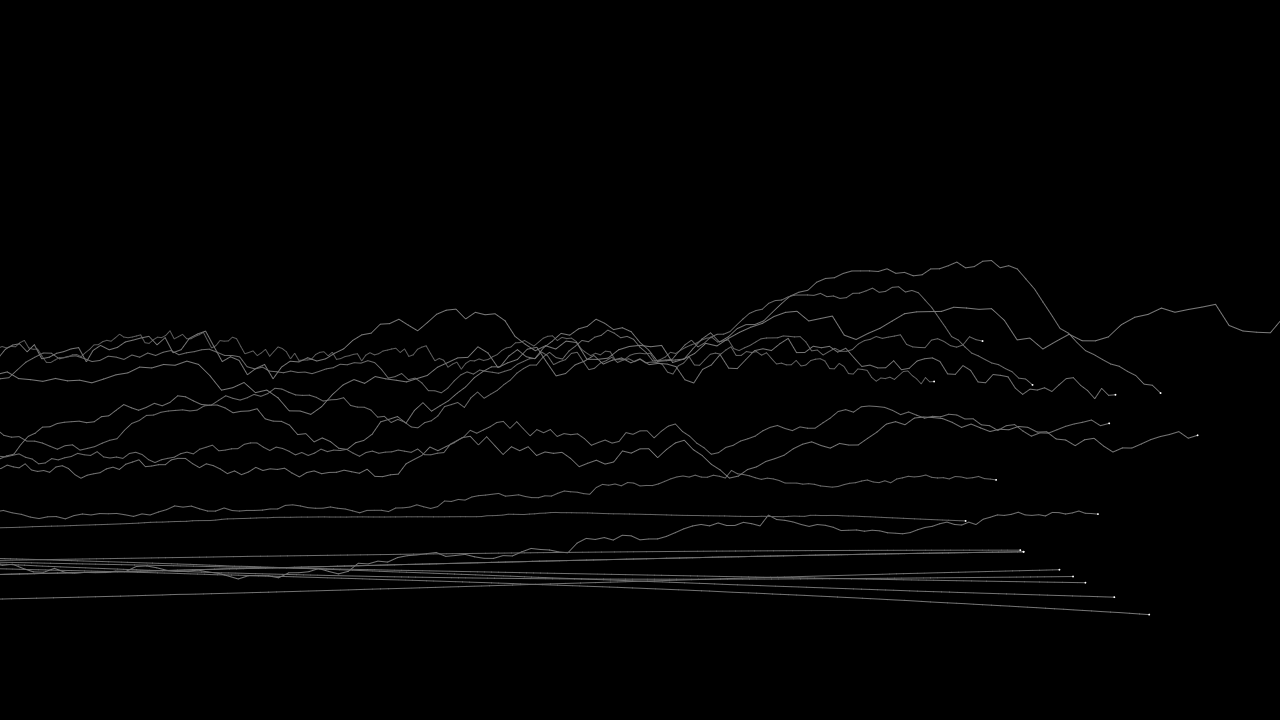
\includegraphics[width = \textwidth ]{Graphs/SpectralWindow.png}
        \caption{Harmoniques dans l'espace}
        \label{SpectralWindow}
    \end{figure} 

    \begin{figure}
        \centering
        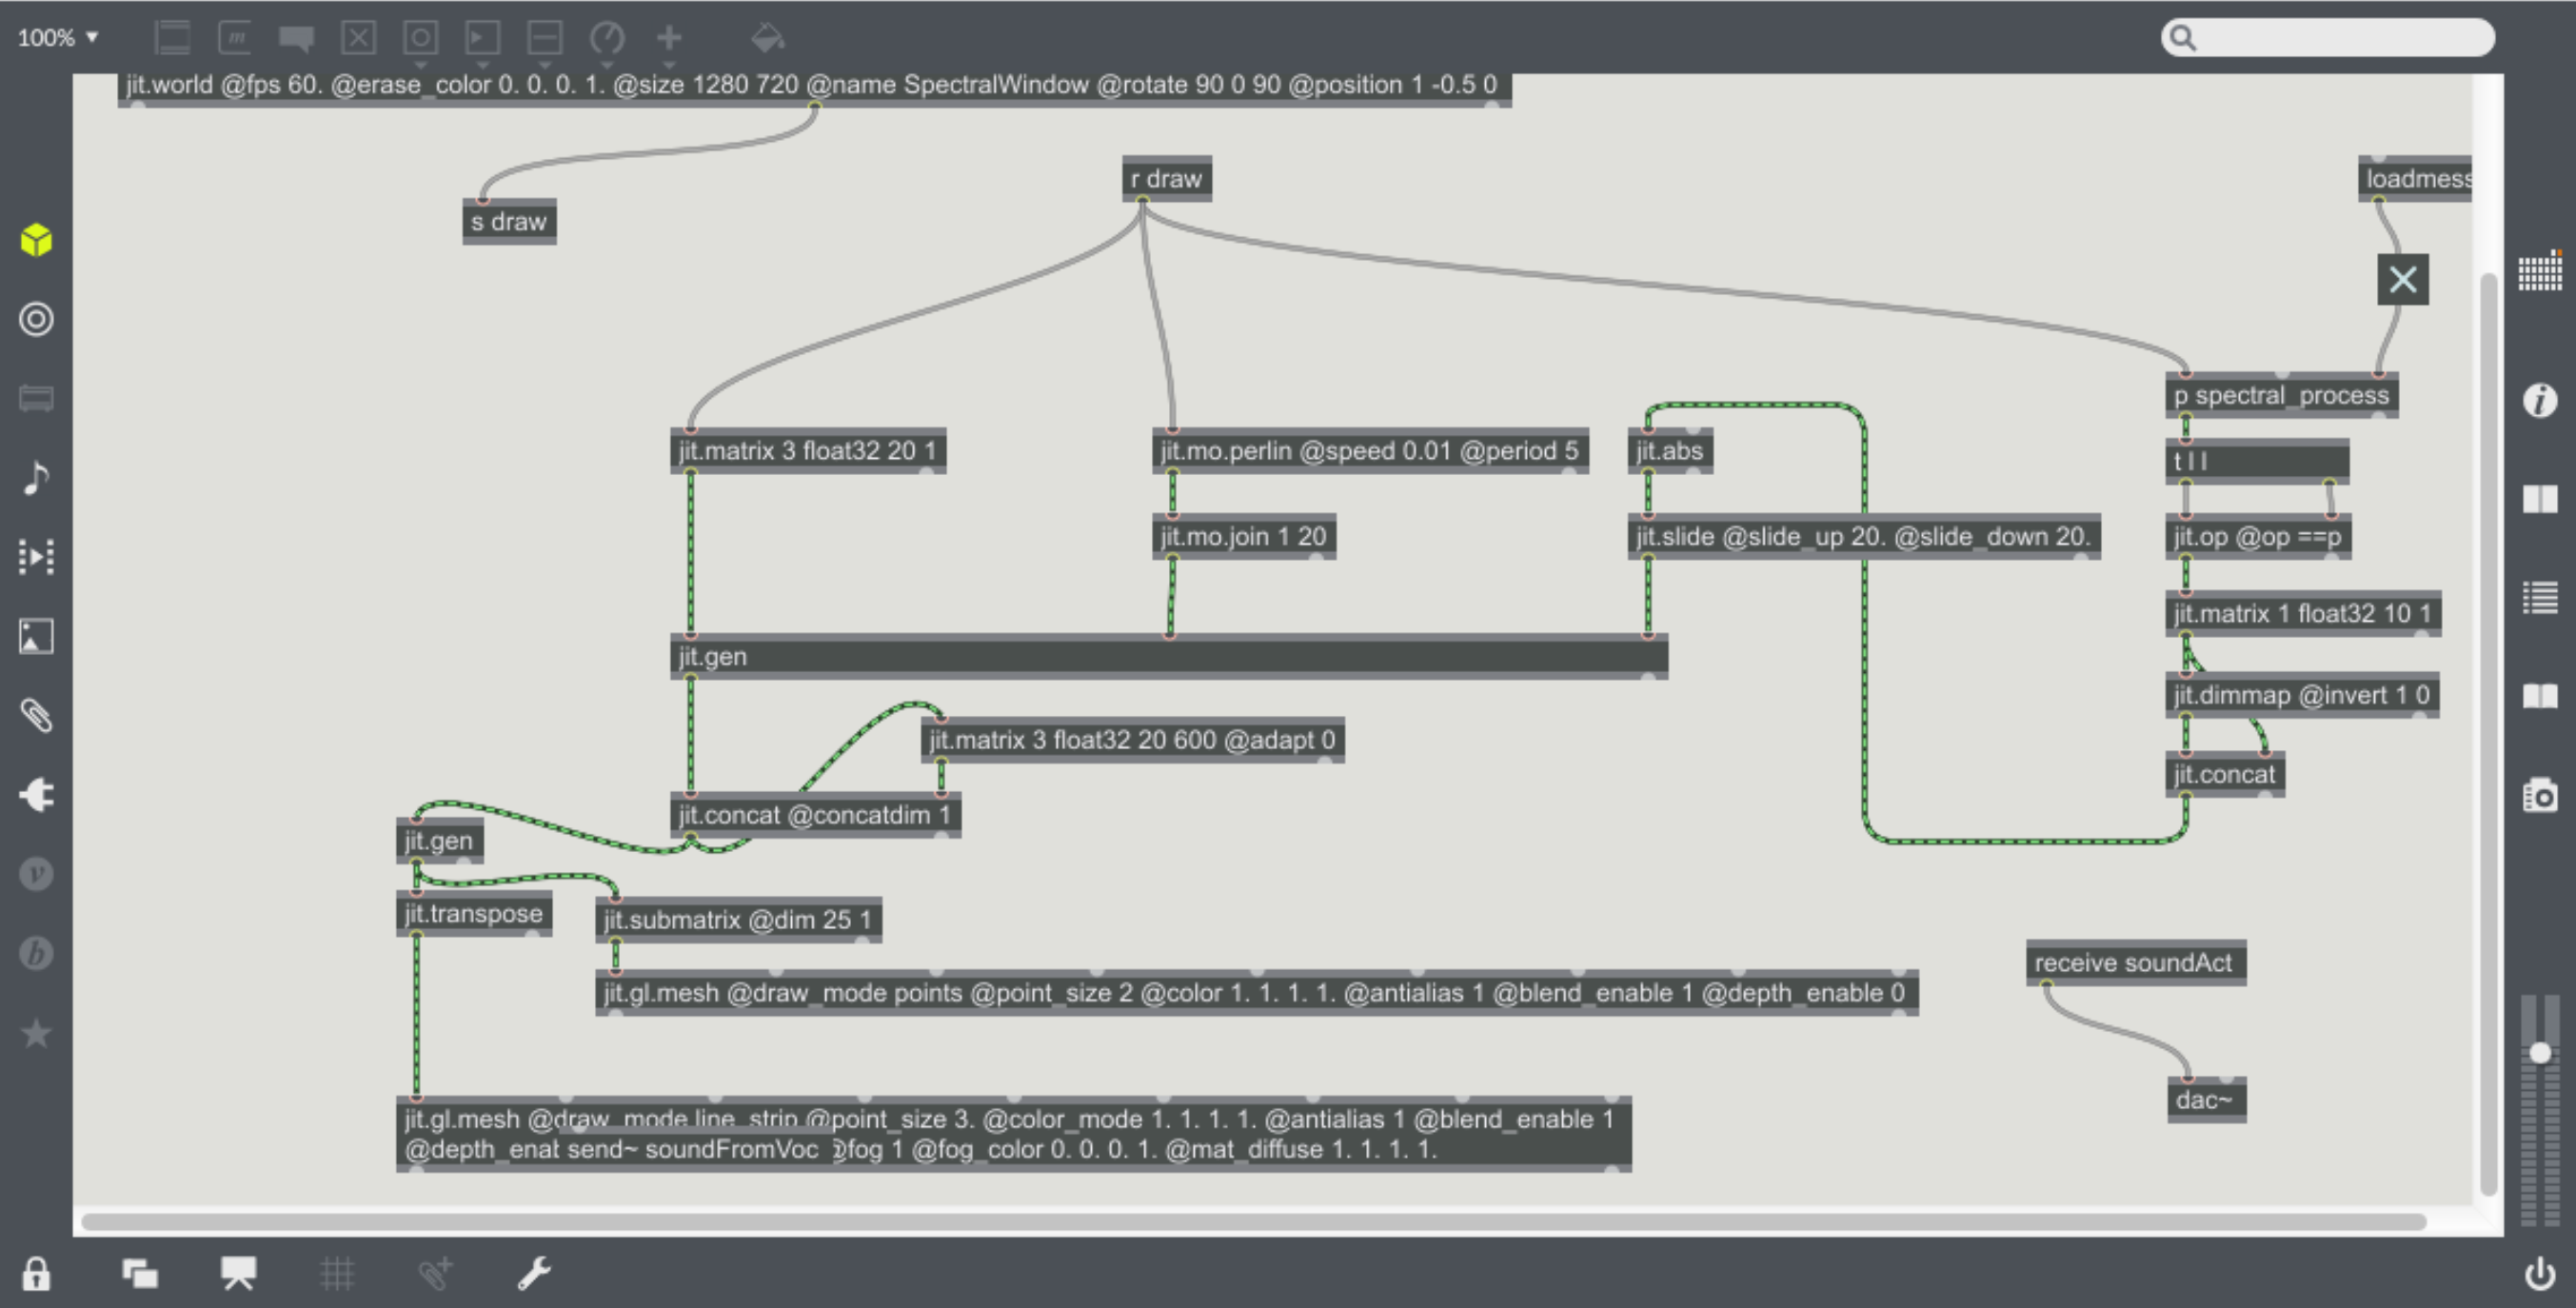
\includegraphics[width = \textwidth ]{Graphs/SpectralDraw.png}
        \caption{Le patch qui control les objets jitter}
        \label{SpectralDraw}
    \end{figure} 


\section{La mise en œuvre compositionnelle}

Dans le cadre artistique, on a créé une composition de courte durée afin de mettre en valeur l'importance artistique du vocodeur de phase via une source d'exemples fructueux. Le but de cette petite pièce de composition est d'utiliser le minimum d'information sonore (3-4 enregistrements de $.<10$ secondes), afin de créer un univers sonore engendré par paramétrisation sur le vocodeur de phase présenté tout au long de ce mémoire.

Chaque son est produit dans Max en utilisant un des codes développés et présentés dans ce mémoire. Chaque son est un produit direct d'un ou deux sources sonores. Les sources sont des enregistrements de piano ou de la guitare effectués et joués par l'auteur. L'orchestration numérique de la pièce était réalisée sur le logiciel du mixage \textit{Reaper}. 

Les enregistrements des sons d'origine étaient faits avec un échantillonnage de $48kHz$ mais les enregistrements dans Max sont reconfigurés à $44,1kHz$. L'enregistrement sur Max est effectué par un \textit{buffer$\thicksim$} et un simple objet \textit{record$\thicksim$}. 

La pièce composée agit d'une pièce acousmatique. L'idée de composition origine de la simulation de l'addition de deux sinusoïdes avec une fréquence différente, mais proche. Ce battement sonore est reflété par des crescendos qui vont et viennent pendant la durée totale de la pièce. Par conséquent, le nom de la pièce est \textit{Diakrotima}, qui signifie battement sonore en grec.

D'une manière quasi régulière les sons se précèdent presque consécutivement. Chaque son est différent et similaire, cela souligne l'existence d'un vocodeur de phase. Cette méthode compositionelle est inspiré par la musique de Morton Feldman \footnote{Hirata Catherine Costello, \textit{The sounds of the sounds themselves: Analyzing the early music of Morton Feldman}, 1996. \nocite{hirata1996sounds}}. "Chaque son comme si presque efface de sa mémoire ce qui est arrivé auparavant", disait Morton Feldman. C'est sur ce dire de Feldman que l'inspiration de cette composition émerge.

    \begin{figure}
        \centering
        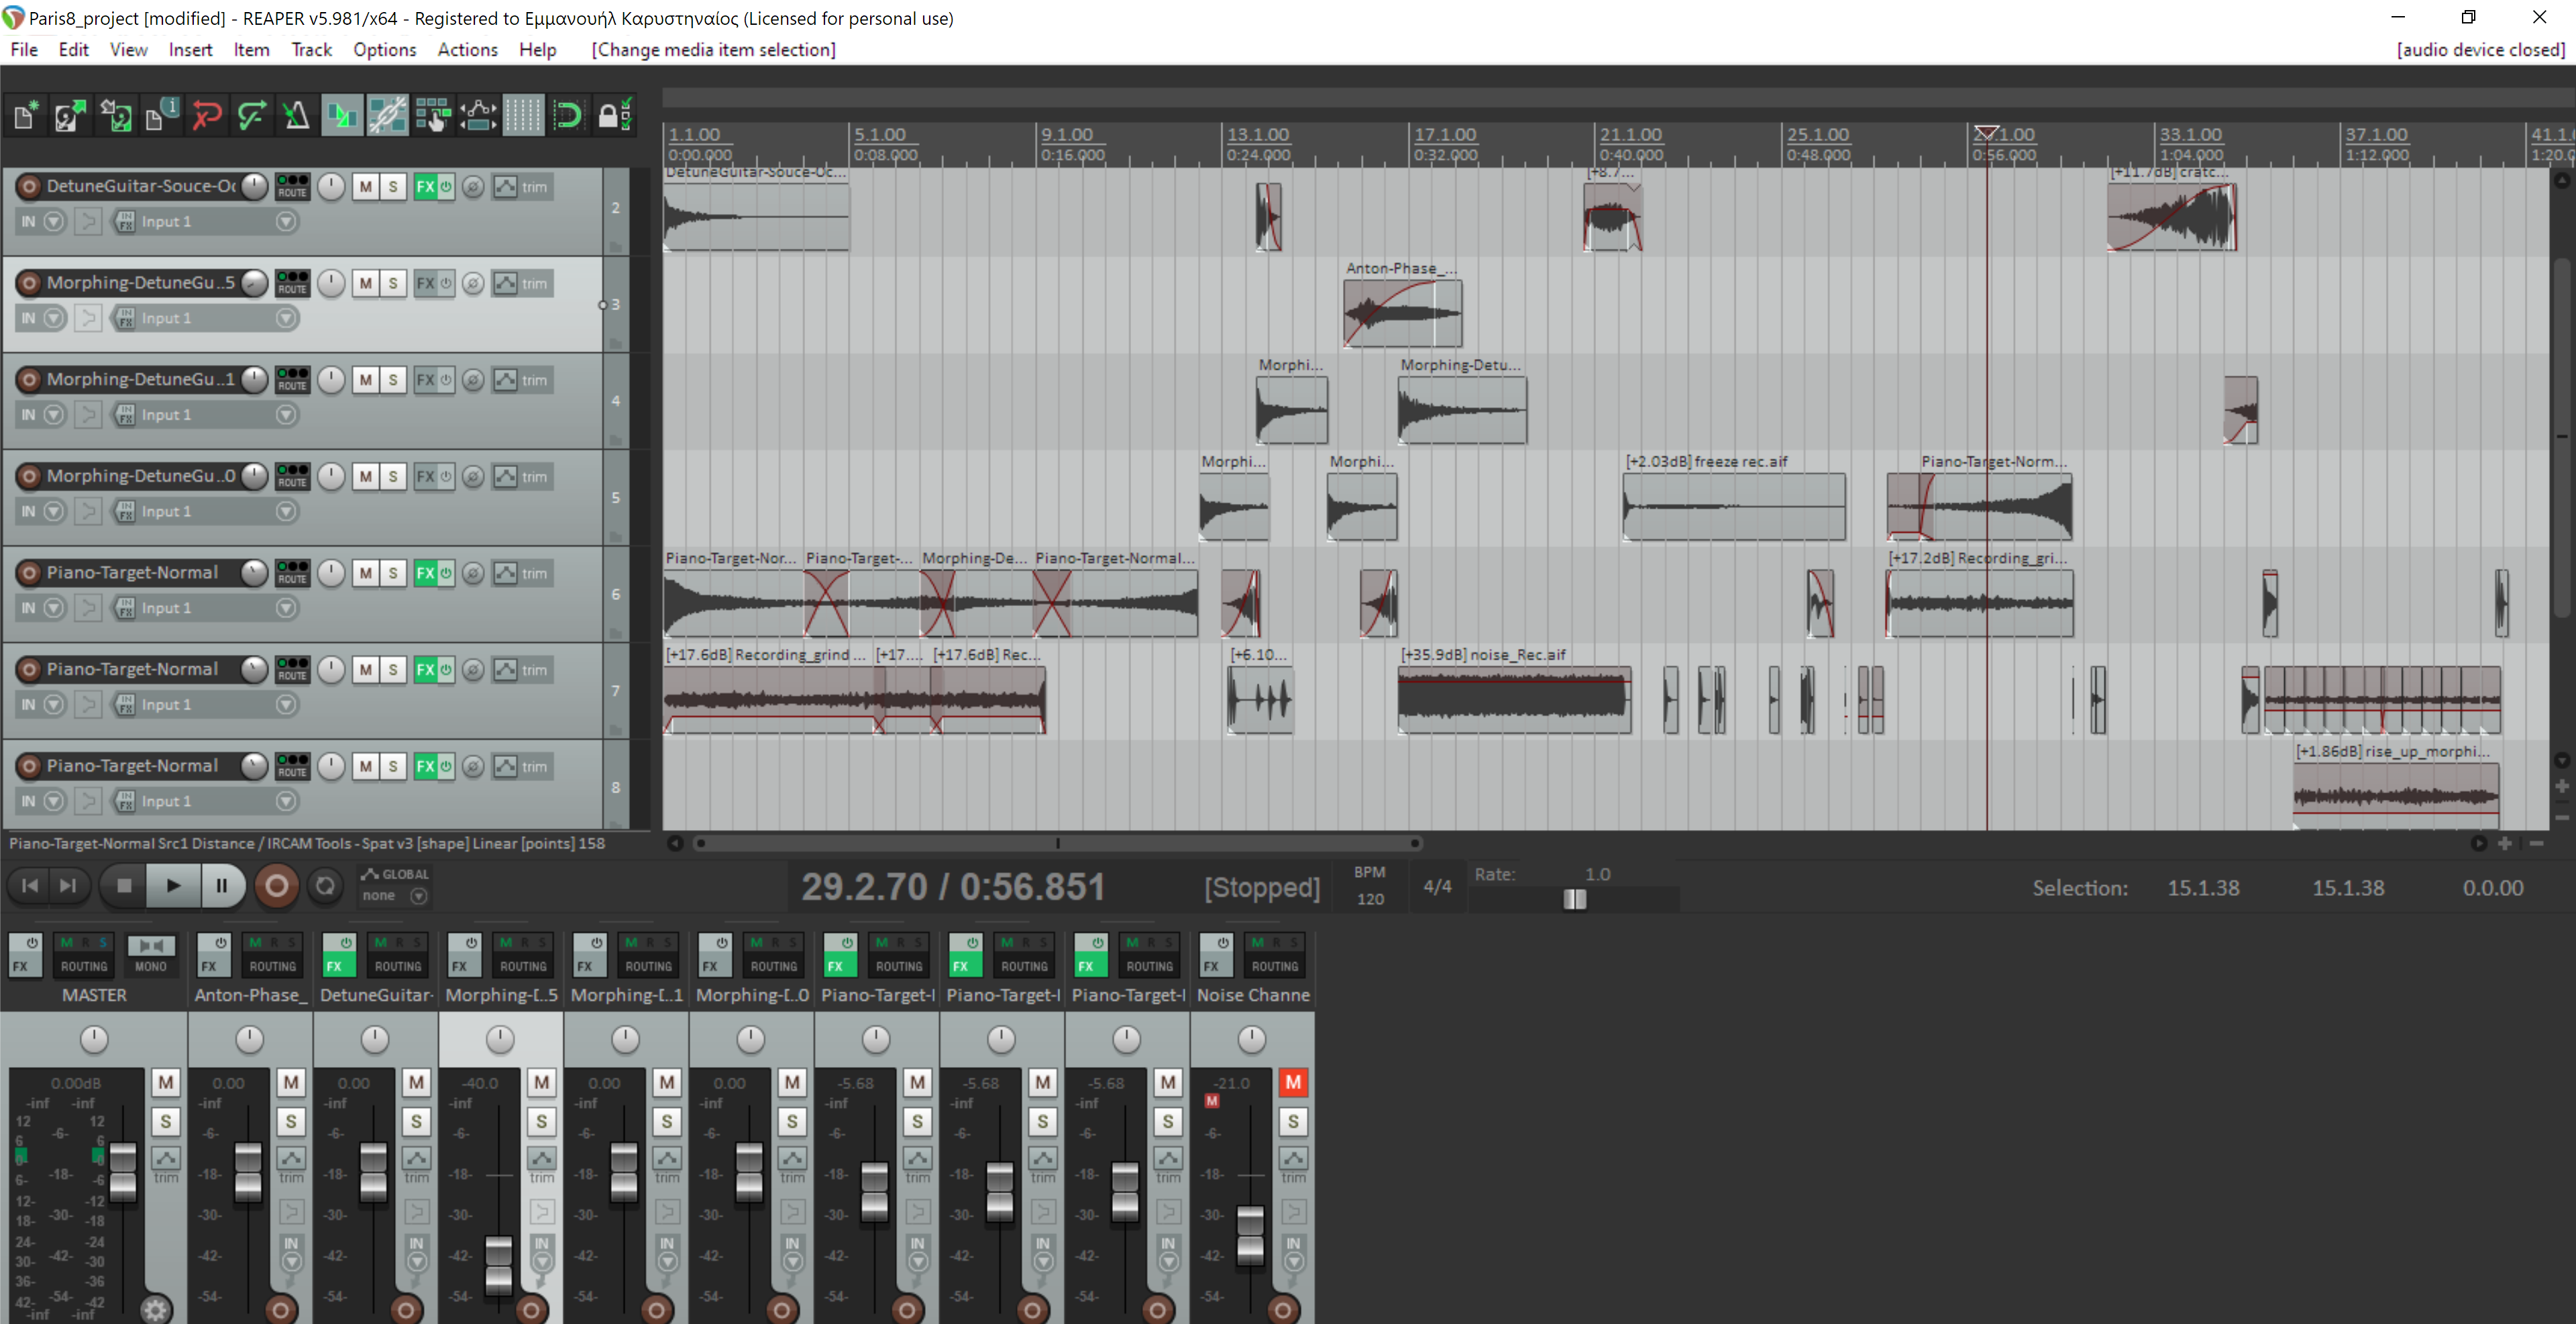
\includegraphics[width = \textwidth ]{Graphs/Reaper_capture_project.png}
        \caption{Partie du mixage de Diakrotima sur Reaper}
        \label{Reaper_capture}
    \end{figure} 

Pendant le processus de mixage les seuls effets complémentaires utilisés sont un de-noiser\footnote{\href{https://www.izotope.com/en/products/repair-and-edit/rx.html}{de-noiser de Izotope serie RX7 }} pour enlever le bruit électromagnétique des enregistrements et un outil de spatialisation \footnote{\href{http://forumnet.ircam.fr/product/spat-en/}{SPAT de Ircam Tools}}. Aucun effet de modification sonore a été ajouté afin d'avoir des sons strictement produits par un vocodeur de phase.

Le format finale de la pièce est un fichier \textit{wav} normalisé en stéréo. La pièce, les enregistrements d'origine aussi bien que les enregistrements de Max sont disponibles sur le repository \href{https://github.com/melkisedeath/Memoire-du-Master-Paris8---Domaines-fondtionnels-du-vocodeur-de-phase}{github} de ce projet de recherche. 

\subsubsection{Analyse structurelle}

La pièce, \textit{Diakrotima}, a une forme asymétriquement périodique conforme à une structure varié et complexe. Le début est fort et dynamique avec un son de source qui a pour origine un enregistrement d'une E2\footnote{la fondamentale presque à $83 Hz$.} de piano joué en forte. En même temps, un son d'origine de frottement avec un plectre sur la sixième corde de la guitare ajoute de la tension bruyant et continue sur la pièce.

La deuxième vague du battement arrive avec une F2\footnote{la fondamentale presque à $87 Hz$.} de la guitare jouée en fortissimo d'une mode pizzicato Bartók. La suite consiste à une modification du même son. Quelques sons percussifs de courte durées sont réalisés par un double vocodeur de phase pour morphing. Les deux sons utilisés sont le pizzicato Bartók à la guitare ainsi qu'un son de frottement avec le plectre. 

La paramétrisation d'un son percutant agit sur une courbe gaussienne du fenêtrage Gabor avec $\sigma$ suffisamment petit, ainsi qu'une transposition de l'un de deux sons vers le registre aigüe. Le patch utilisé est le \textit{Super Phase vocodeur} contenant du morphing, de la transposition, du freeze et du changement de la temporalité. Pour construire plus des sons à base du bruit, on construit une courbe gaussienne très serré avec $\sigma \simeq 0$, l'amplitude du bruit au maximum avec $\alpha = 1$ et un freeze temporel.

Tout autre son présenté dans la pièce est une variation du paramétrage. Parfois, on choisit de mélanger des modifications percutantes de sons avec une transposition de la hauteur. Les autres produits sonores sont de la variation des valeurs de phase et d'amplitude parmis le \textit{Super Phase Vocoder}. 

\subsection{L'évaluation artistique}

Dans le cadre de recherche, il s'agit d'une suite logique d'application de la critique de l'œuvre. Ici, donc, on se focalise sur un point de vue épistémologique, de l'évaluation de la mise en œuvre, des applications du vocodeur de phase dans ce contexte artistique. 

Dans la pièce \textit{Diakrotima} se trouve une palette des sons produits exclusivement par un vocodeur de phase avec très peu de matériel sonore à l'origine. On a pu ainsi demontré que les possibilités d'un vocodeur sont presque infinies dans un contexte artistique, mais on remarque encore quelques défauts. 

Quand on applique un changement de la hauteur plus d'une octave vers le bas, on retrouve une perte de qualité considérable. Également, si un son n'est pas très harmonique, au sens qu'il contient des caractéristiques très percutants et qu'il n'a pas de fréquence persistante, on se rend compte que toute opération de changement de la hauteur ou du rythme de lecture n'est pas optimale. Au-delà des problèmes techniques liés à la construction de l'algorithme, on peut constater que les sons produits avec le vocodeur de phase ont tous un caractéristique rond. C'est-à-dire que l'effet de reproduire de sons à partir des sinusoïdes donne l'impression que tout son est similaire et par extension pas naturel. 

L'effet d'avoir des sons arrondis ou artefacts est parfois bien désirable. Pour autant, le résultat reste toujours robuste et de haute qualité. Or, le vocodeur de phase ne semblerait pas être le premier choix des outils informatiques pour des compositeurs qui souhaiteraient créer des pièces acousmatiques avec des sons d'une haute qualité réaliste.